\begin{figure}
\begin{fullwidth}
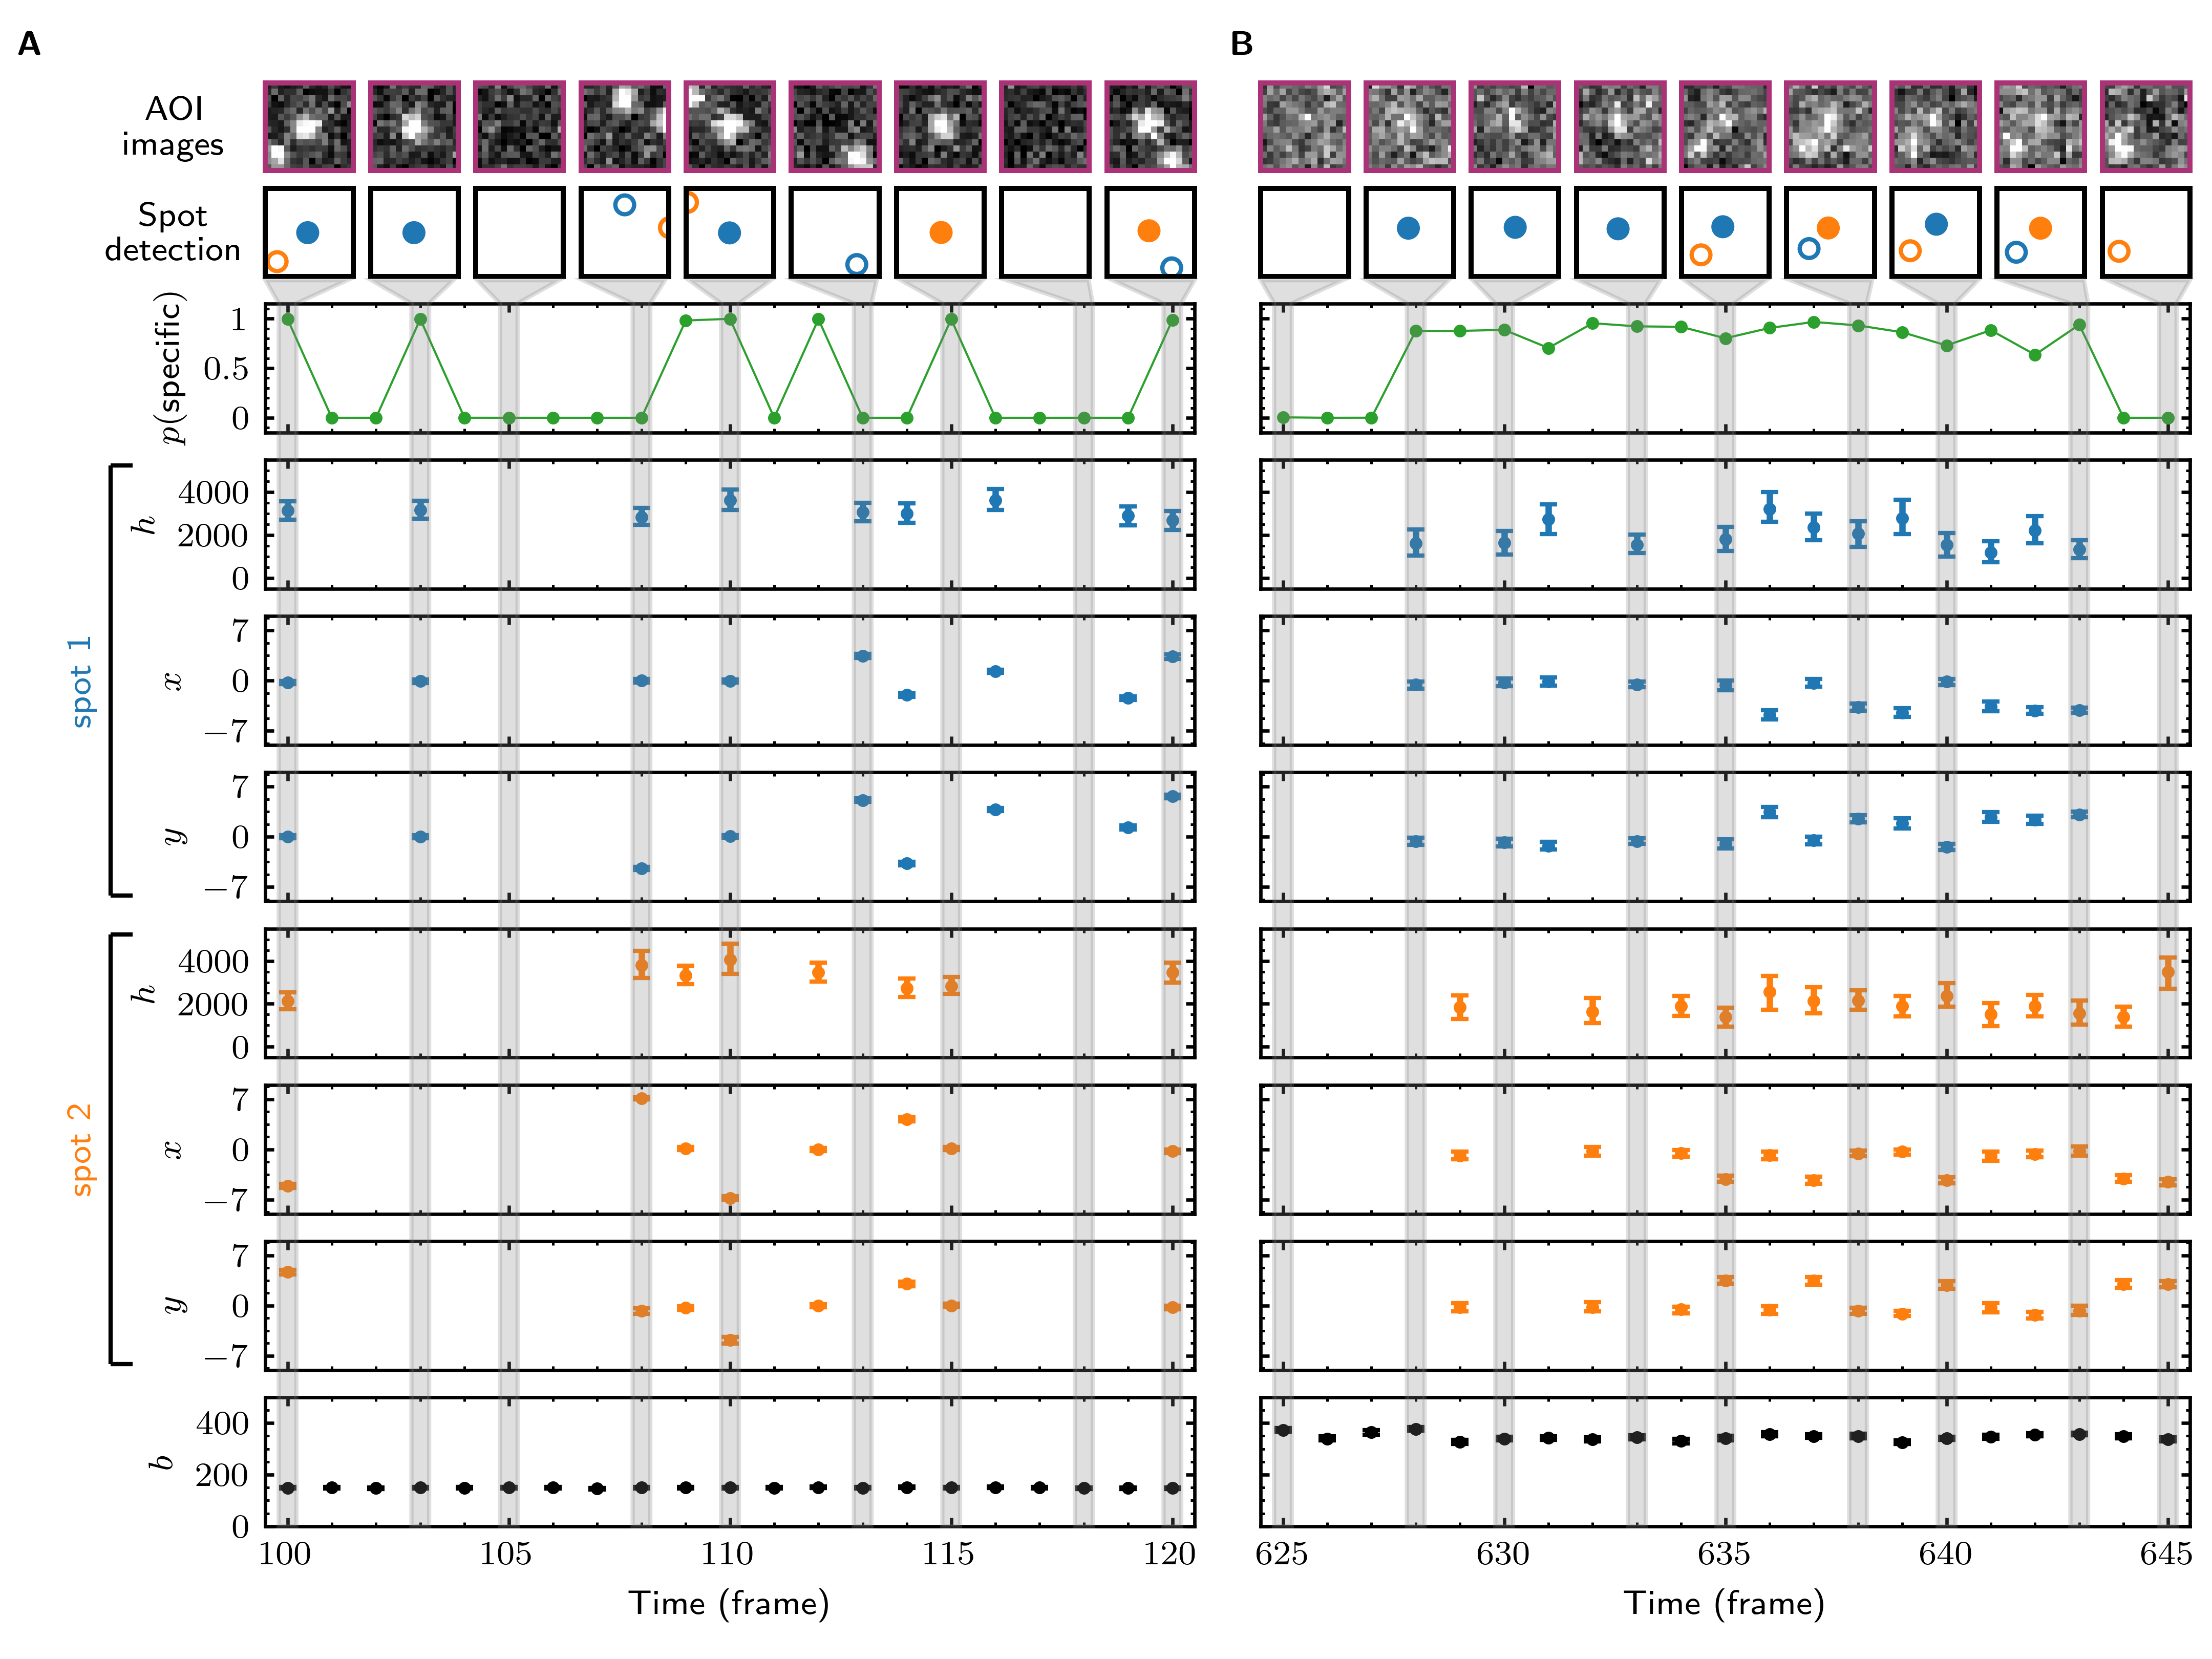
\includegraphics[width=183mm]{figures/tapqir_analysis.png}
\caption{\textbf{Tapqir analysis and inferred model parameters.} (\textbf{A},\textbf{B}) Tapqir was applied to simulated data (\texttt{lamda0.5} parameter set in Supplemental Data 1) (\textbf{A}) and to experimental data (Data set A in \TABLE{datasets}) (\textbf{B}). (\textbf{A}) and (\textbf{B}) each show a short extract from a single target location in the corresponding data set. The first row shows AOI images for the subset of frames indicated by gray shaded stripes in the plots. The second row shows the locations of spots determined by Tapqir. Spot numbers 1 (blue) and 2 (orange) are assigned arbitrarily and may change from fame to frame. Only data for spots with a spot probability $p(m=1) > 0.5$ are shown. Spots predicted to be target-specific ($p(\theta=k)>0.5$ for spot $k$) are shown as filled circles. The graphs show the probability of there being any target-specific spot in a frame ($p(\mathsf{specific})$; green), spot intensity ($h$), location ($x$, $y$) of spot 1 (blue) and spot 2 (orange), and AOI background intensity ($b$). Error bars: 95\% CI (credible interval).}
\label{fig:tapqir_analysis}

\figsupp[Tapqir analysis and inferred spot probabilities.]{\textbf{Tapqir analysis and inferred spot probabilities.} The first two rows and $p(\mathsf{specific})$ graph are as in \FIG{tapqir_analysis}. The new graphs show the probability of a spot being target-specific ($p(\theta=k)$ for spot $k$) and the probability of spot presence ($p(m=1)$) of spot 1 (blue) and spot 2 (orange).}{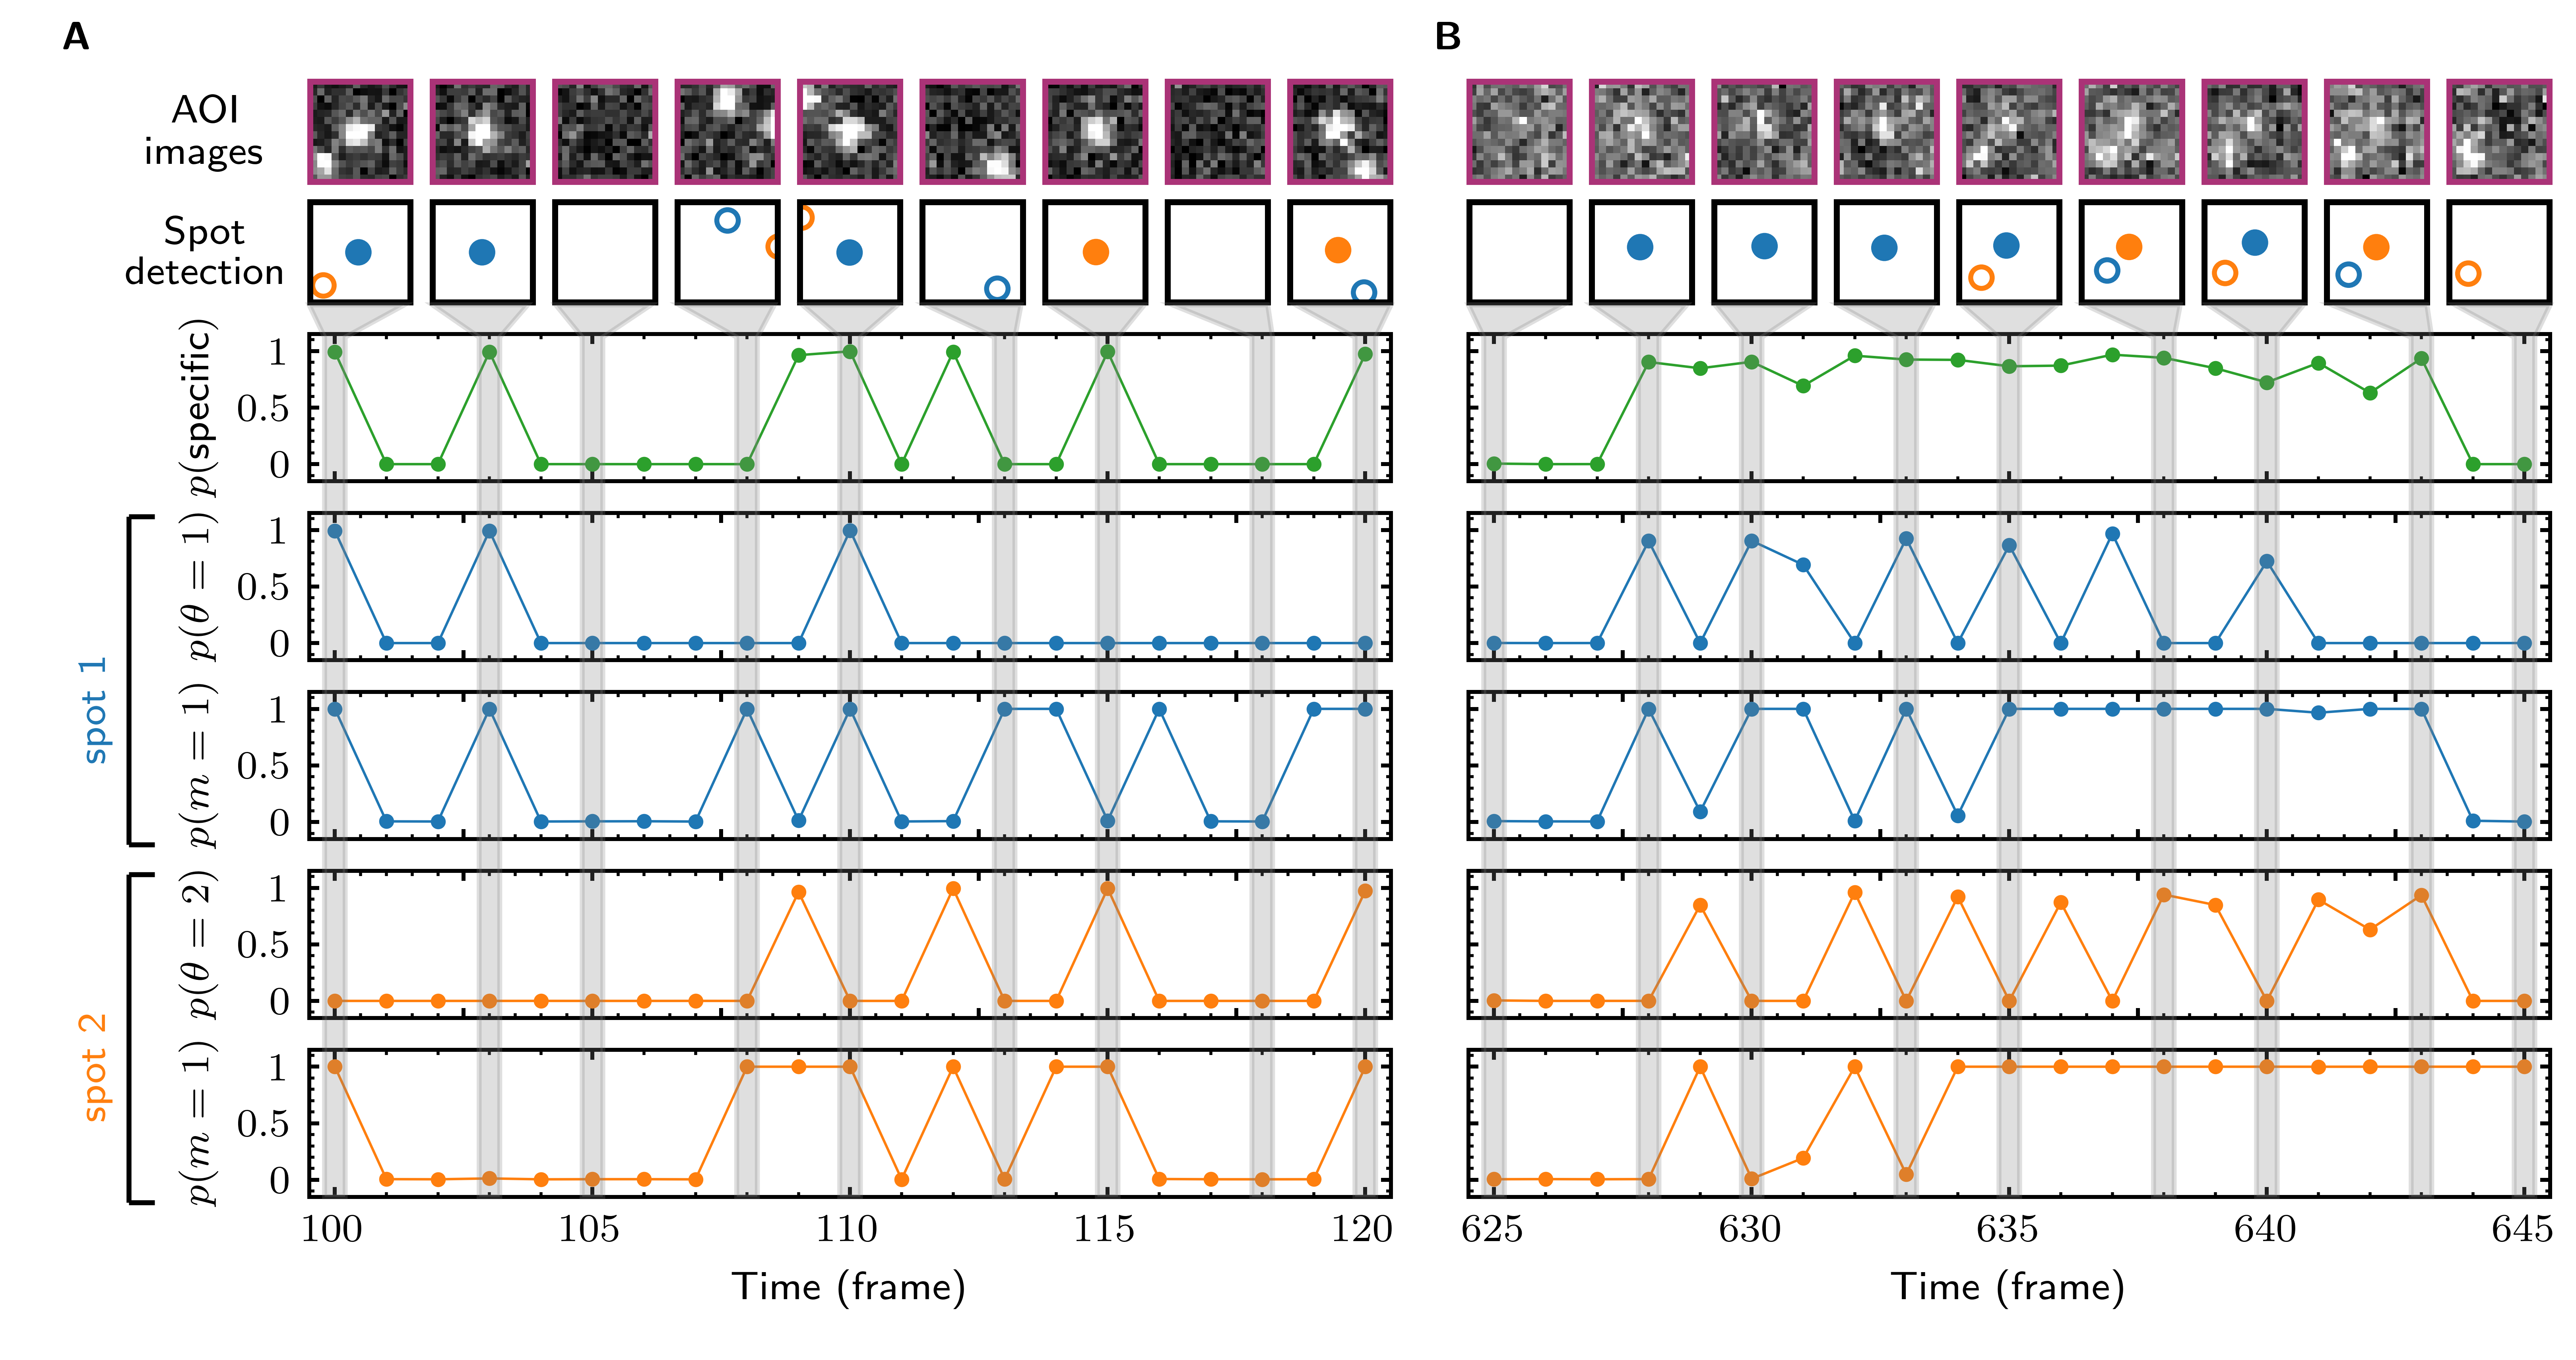
\includegraphics[width=183mm]{figures/tapqir_analysis_probs.png}}\label{figsupp:probs}
\figsupp[Reproduction of experimental data by posterior predictive sampling.]{\textbf{Reproduction of experimental data by posterior predictive sampling.} Example frames are shown from Data set A  (\textbf{A}: SNR = 1.63), Data set B (\textbf{B}: SNR = 3.43), Data set C (\textbf{C}: SNR = 4.18), and Data set D (\textbf{D}: SNR = 3.14) in \TABLE{datasets}. In each panel the top row shows AOI images selected from the experimental data and middle row shows corresponding images obtained by sampling from the posterior distributions. The bottom row shows pixel intensity distributions from the experimental and posterior prediction images shown.}{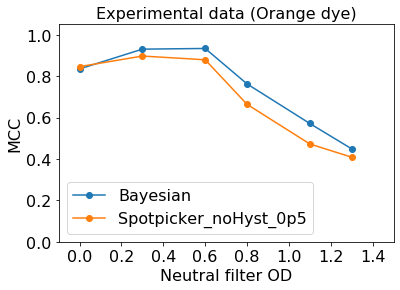
\includegraphics[width=183mm]{figures/figure4.png}}\label{figsupp:ppc}

\figsupp[Tapqir analysis of image data simulated using a broad range of global parameters.]{\textbf{Tapqir analysis of image data simulated using a broad range of global parameters.} Simulations (see Methods) consist of 16 data sets where values of global parameters ($\pi$, $\lambda$, $\sigma^{xy}$, and $g$) where randomly generated for each data set (Supplemental Data 2). Simulated data were fit with Tapqir, and parameter values from the fit (with 95\% credible interval) are plotted against the true parameter values. To guide the eye, dashed lines  indicate identical true and fit values. (\textbf{A}) Gain of the camera $g$. (\textbf{B}) Average specific binding probability $\pi$. (\textbf{C}) Nonspecific binding rate $\lambda$. (\textbf{D}) Proximity parameter $\sigma^{xy}$.}{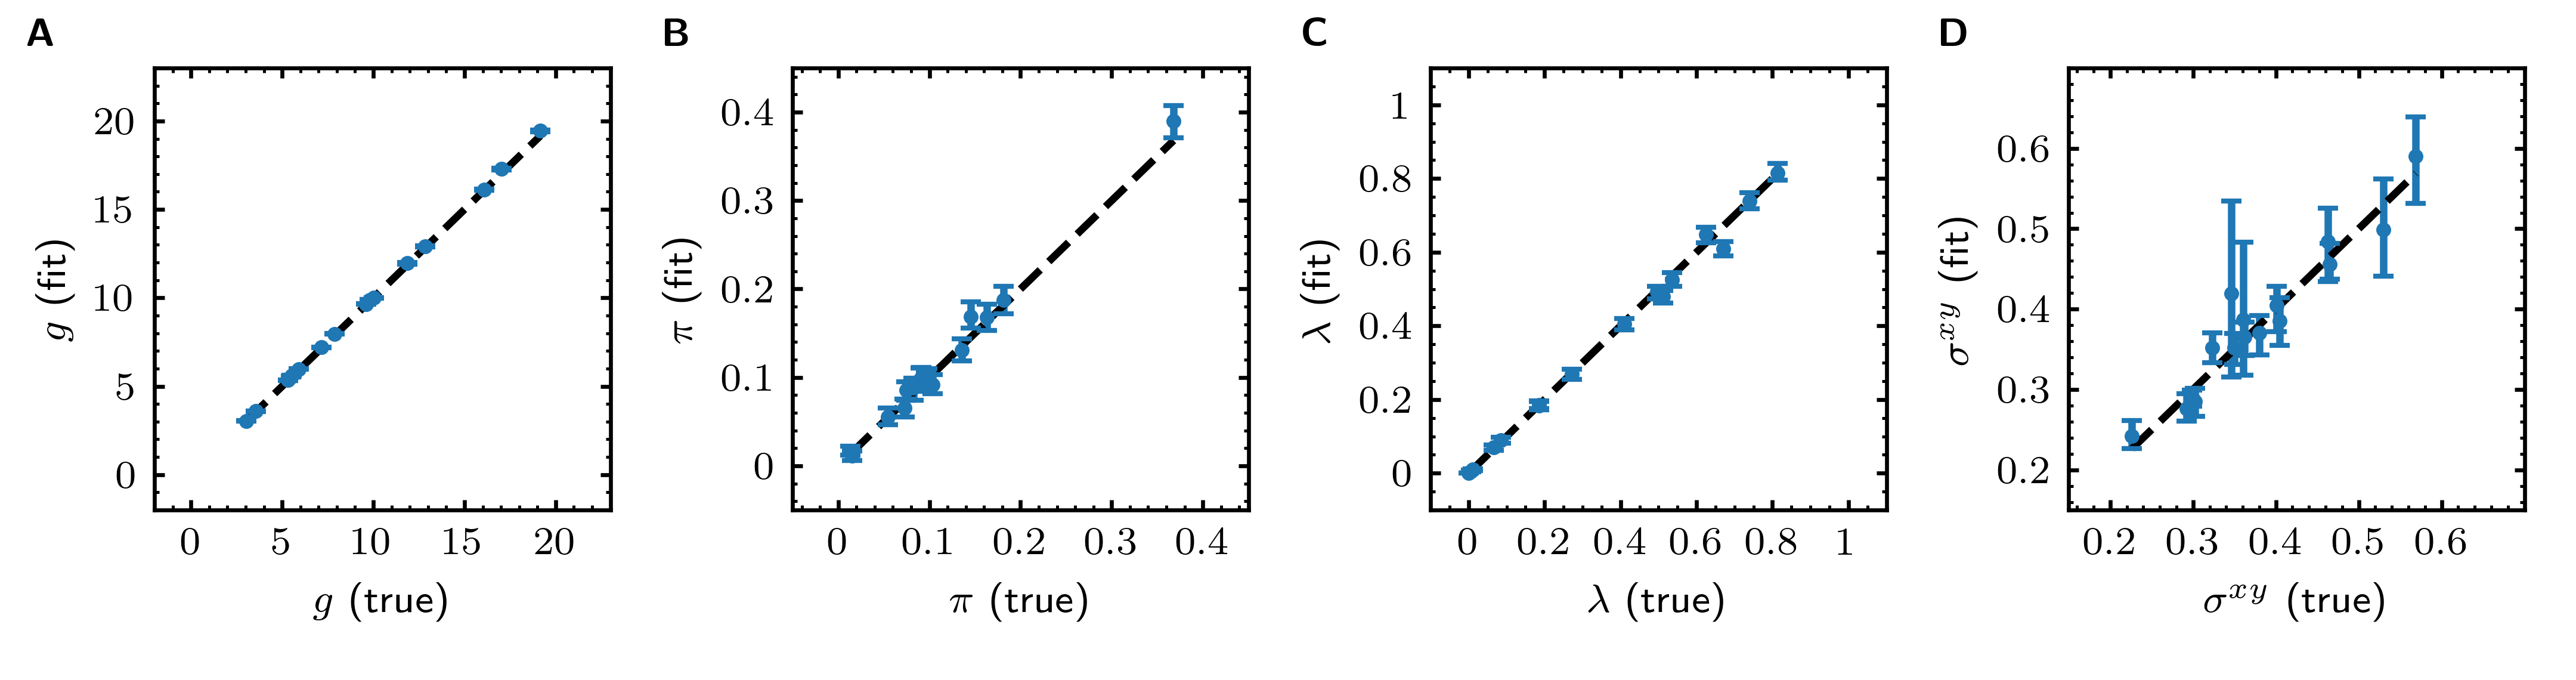
\includegraphics[width=183mm]{figures/tapqir_analysis_randomized.png}}\label{figsupp:randomized}
\end{fullwidth}
\end{figure}